As users develop models for different sources, they can publish their models in a repository to share with other users.  
This repository can also serve as a collaboration point for users to subsequently build upon previously published models.  
Karma users can use the interface illustrated in Figure~\ref{fig:model-manager-screenshot} to add models from external sources by providing a URL or remove models that are obsolete or otherwise no longer useful.  
Figure~\ref{fig:model-manager-screenshot} also enumerates a number of models for data from the Smithsonian that were developed against csv files generated from database table samples.  
When users want Karma to generate RDF from a future source, they can also apply an appropriate model from the repository.

\begin{figure*}
\begin{center}
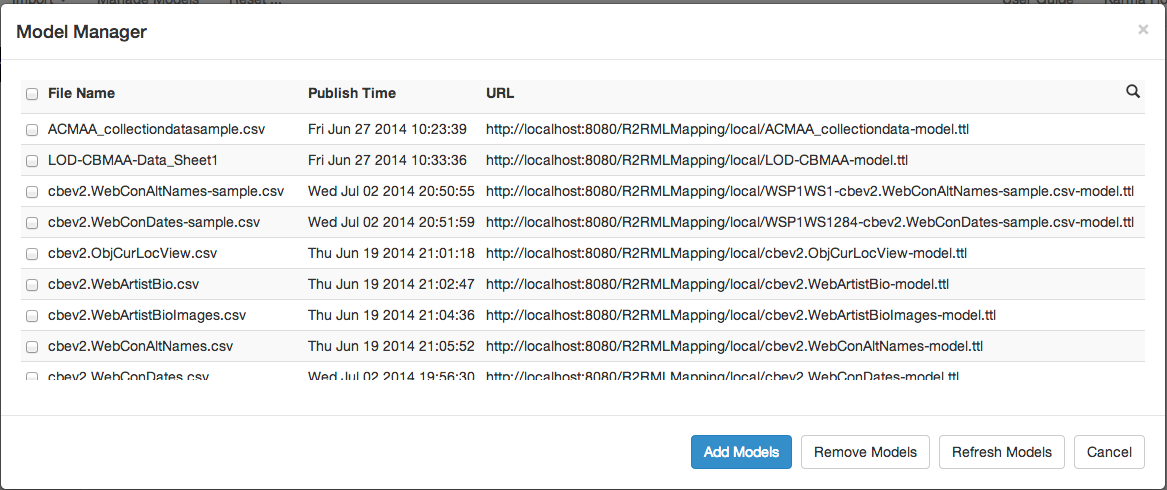
\includegraphics[width=4.0in]{3-model-manager.png}
\vspace{-3mm}
\caption{A list of source models a user has made available to Karma}
\vspace{-2mm}
\label{fig:model-manager-screenshot}
\end{center}
\vspace{-1.5em}
\end{figure*}

